\chapter{Vision}
The Vision module is responsible for controlling the camera and to publish estimated positions based on seen AR markers. It also notifies the system about any unexpected markers.

\label{Vision chapter}
\section{Working Process}
\subsection{Overview}

We began our project by becoming familiar with ROS, going through  several tutorials on it and setting everything up. In the second step we studied the Kinect along with its functions and possible applications. Next we started integrating \texttt{ar\_track\_alvar} -- AR tag tracking library -- into our project, implemented marker recognition and tracking.Figure \ref{AR tags} shows example tags. Finally we tested the behavior intensively. \\
\begin{figure}
\begin{center}

\includegraphics[width=\linewidth]{graphics/markers.png}
\caption{AR tags}
\label{AR tags}
\end{center}
\end{figure}
In an effort to find the optimal conditions for marker recognition, we tested bundled markers as well as single markers per location (we were limited by the size of an A4 page).

The Kinect's field of view is relevant for this as well, so we determined the maximum possible distance and angle for marker recognition. After generating markers and ensuring their correct and reliable detection, we started working on receiving transform information from \texttt{ar\_track\_alvar} and learned how to interpret it in ROS. We derived world coordinates from it according to the coordinates of the robot and calculated covariances for them.

Afterwards we put our hands on the \textit{Pan-Tilt Unit (PTU),} a device used for head movement. PTU drivers needed to be installed on the computer and its settings were configured. We became accustomed to the basics of PTU movement and designed an efficient algorithm to let the head continuously follow a seen marker, in doing so maximizing the time the robot is in contact with markers.

In the final step we implemented logic for publishing the next expected marker based on the current estimated position. All required markers were generated and placed on walls with fixed distance from each other and simple database including all markers along with their position was built.

During testing we encountered various expected and unexpected problems as well as bugs. We spent a significant amount of time resolving them and finding an appropriate solution for each problem. Although some of them consumed a lot of time to solve, they mostly helped us acquire new knowledge.

\subsection{Tasks assignment}

Starting from October we worked hard to achieve our goals. Our team was formed out of three people, Valeriy Gatuzov, Codrin Goia and Guilherme Pires. Guilherme has returned to his home country at the time of writing, he made his contribution to the documentation separately by writing in the project wiki, so his work will only be briefly discussed here. From the beginning we divided all incoming tasks equally in the group, so that everyone could make a good contribution to the project. Below we outlay the differentiation of tasks in the group:

Guilherme brought extensive knowledge and experience in Linux systems with him, the remaining two of us needed to learn it at first. As we started working on \texttt{ar\_track\_alvar}, Guilherme and Valeriy integrated it into the ROS environment and set it up. At the same time Codrin worked on the data processing from \texttt{ar\_track\_alvar}. He learned a lot about TF-Trees and \texttt{ar\_track\_alvar} itself. Later on he developed an algorithm for transforming local coordinates from markers sent by \texttt{ar\_track\_alvar} to world coordinates and to publish them to the other groups.

Meanwhile Valeriy calibrated marker recognition, generated markers and worked himself through all sorts of errors delegated to him from other teammates. Later on Guilherme implemented an algorithm for computation of the covariance. Valeriy started working on tracking markers with the Pan-Tilt Unit and was challenged with problems like finding an appropriate mathematical function to implement the movement, calibrating the turning speed, stopping the head on time, and at testing and debugging it.

Almost at the end we worked on the next expected marker problem, discussed the details and all possible solutions, then made a concept algorithm, that was implemented by Guilherme and Codrin. Then Valeriy  tested the entire software, writing a testing program and resolving new-found errors. Codrin concentrated on an unexpectedly appeared problem concerning the computation of coordinates which he successfully fixed.  

\subsection{Used Resources} 

We used a lot of open source resources, that were essential to our success. From the beginning we learned a lot about Linux, because we did not have much experience in it. Then we became familiar with ROS, its packages, nodes, core commands and its functioning principle in general. We learned all the concepts starting from catkin and roscore, all the way up to tf. As a visualizalation and debugging tool rviz was very helpful for verifying e.g. if axes direction are correct. rqt\_graph helped us understand the connection between different nodes. We successfully employed the Kinect in our work for recognition of markers which were generated with \texttt{ar\_track \_alvar} -- an open source AR tag tracking library for ROS. We used ``createMarker'' -- another useful tool and part of \texttt{ar\_track\_alvar}, that helped us create a graphical representation for bundles of markers as well as for single markers. Each time it generates an XML file for it. Later on, when we started working with Pan-Tilt Unit for the purpose of moving the head, we installed \texttt{flir\_ptu\_driver}, \texttt{ptu46} and \texttt{ptu\_control} in order to be able to control the PTU.

\section{Conceptual Design}

\subsection{Components}
At a conceptual level, the Vision package can be decomposed in two components, implemented in two ROS nodes: \texttt{localizer} and \texttt{marker\_broadcaster}. The internal interaction between them and all other external nodes does not need to be understood or changed from the exterior, as the whole setup is launched in the custom \texttt{vision.launch} file of the package Vision.
The \texttt{marker\_broadcaster} node is responsible for feeding the tf system with the position of all markers inside the database. \texttt{localizer}, being the node containing the main functionality, deals with the processing of data from the Kinect camera and uses the tf data from \texttt{marker\_broadcaster} in order to output a position with covariance. Figure \ref{Vision Concept} shows how the data flow inside the Vision package undergoes several transformations in order to output the position of the camera:

\begin{figure}[h]
\begin{center}
\includegraphics[width = \linewidth]{graphics/vision_concept.png}
\caption{Transformations from input to outpout}
\label{Vision Concept}
\end{center}
\end{figure}

Since the navigation will only take place in one plane which the robot will never leave, all the 3D data is filtered out as soon as possible to keep computations at the appropriate level and to avoid computation of unnecessary data. This takes place immediately after the interpretation of marker position coming from \texttt{ar\_track\_alvar}. From that point on coordinates in the whole system will only have 3 values, namely x coordinate, y coordinate, and rotation around z-axis. 

\subsection{Dependencies}
The main purpose of the Vision group is to collect data coming from the Kinect camera, process it and output a data in form of a position on the map. Secondary purposes are the signalization of a seen marker, signalization of an unexpected marker, as well as commands to the Pan-Tilt Unit rotation in order to rotate the head towards the seen or expected marker. In other words, the role that the vision package plays is to serve as a mediator between external ROS nodes feeding it with raw data and generating useful data for the Kalman and High Level Components to process. In order to be able to work, all external dependencies need to be present when being launched. At a conceptual level, these dependencies are:

\begin{enumerate}
\item External ROS packages publishing from outside the project:
\begin{itemize}
\item \texttt{freenect\_launch} for collecting data from the Kinect camera
\item \texttt{ar\_track\_alvar} for processing image data from \texttt{freenect\_launch} and output marker positions
\item \texttt{flir\_ptu\_driver} for managing camera rotation
\end{itemize}
\item Internal ROS packages publishing from inside the project: 
\begin{itemize}
\item High Level
\item Kalman
\end{itemize}
\item Marker positions database in form of a text file.
\end{enumerate}

\subsection{Interactions with other Groups}
Information between the Vision package and the other components of the project is done using the standard ROS messages. The main node from the Vision package publishes pose information coming from higher level nodes of Kalman and High Level group and subscribes to the incoming processed data coming from them.

\begin{description}
\item Output topics:
\begin{itemize}
\item vision/estimated\_pose topic: main topic, in which the position of the robot with respect to world coordinates is published
\item vision/sees\_marker topic: is publishing only when a marker has been seen. 
\item vision/unexpected\_marker  topic: it is intended to serve as a trigger to High Level group in order to signalize that a kidnapping might have occurred.
\end{itemize}
\item Input topics:
\begin{itemize}
\item HL/is\_kidnapped topic: In case of a kidnapping, the camera rotation enters a searching state, where it is constantly spinning in search of a new marker.
\item kalman/fused\_pose topic: represents the final estimate of the robot position and is used in the computation of the next expected marker in case no kidnapping situation is active. By knowing the estimated position, the location of the nearest marker can be computed and in case nothing is seen, the camera rotates towards that direction.
\end{itemize}
\end{description}

\section{Implementation}

\subsection{Input/Output Specification}
The Vision package communicates with other ROS nodes exclusively through topics. There are input and output ports, local topics that stay within the project to communicate with other teams, and global topics that go outside the project to reach for data input and to send commands.

\begin{itemize}
\item geometry\_msgs::PoseWithCovarianceStamped: output internally to topic ``vision/estimated\_pose''. Represents the main functionality of the vision package, i.e. to provide global robot coordinates computed from camera input and marker database.
\item std\_msgs::Bool: output internally to topic ``vision/sees\_marker''. Is publishing true whenever a marker is identified by the Kinect camera.
\item std\_msgs::Bool: output internally to topic ``vision/unexpected\_marker''. Is publishing whenever the position it receives from Kalman group does not match with the currently seen marker
\item std\_msgs::Bool: input internally from topic ``HL/is\_kidnapped''. Used to decide the camera rotation strategy: whether it shall rotate in search of a marker, or rotate towards expected marker on the map.
\item geometry\_msgs::PoseWithCovarianceStamped: input internally from topic ``kalman/fused\_pose''. Used to determine the distance, direction and finally the ID of the next expected maker.
\item ar\_track\_alvar\_msgs::AlvarMarkers: external input from topic ``ar\_pose\_marker''. Receives seen marker ID and transform in camera coordinates.
\item sensor\_msgs::JointState: external input from topic ``joint\_states''. Used to read the current angle between camera and robot.
\item sensor\_msgs::JointState: output externally to topic ``ptu/cmd''. Used to pass commands to the PTU unit when rotating toward next expected marker or when tracking the currently seen marker.
\end{itemize}

\subsection{Class Dependencies}
In order to collect the image data coming from the Kinect, process it and output a position with covariance, several classes of the ROS library are used. A diagram showing all dependencies can be seen below in figure \ref{Vision Dependencies}.

\begin{figure}
\begin{center}
\includegraphics[scale = 0.8]{graphics/vision_dependencies.png}
\caption{Class dependencies inside Vision Package}
\label{Vision Dependencies}
\end{center}
\end{figure}

\subsection{Package Diagram}
Since the Vision package serves as a link between low level input data in form of image stream and output in form of position, it heavily relies on foreign packages for data acquisition and processing as illustrated in figure \ref{Vision Package Diagram}. Note that the arrows indicate the flow of data inside the topics (from publisher to subscriber), that means arrowheads are positioned exactly opposite to dependency relationships.

\begin{figure}
\begin{center}
\includegraphics[scale = 0.6]{graphics/vision_package.png}
\caption{Flow of data between packages}
\label{Vision Package Diagram}
\end{center}
\end{figure}

\subsection{TF Tree}
In order to position the robot correctly in the world, the tf data between all known coordinate systems is put together in order to compute the missing link: the transform of the robot in world coordinate system. The localization process is initiated only when a marker is seen and consists of two stages, each one implemented in its own thread.

First step: When a new marker is seen by \texttt{ar\_track\_alvar}, the transform of the marker with respect to the camera is converted into 2D in order to get rid of unused data. The inverse is then applied on the transform so that it now represents the position of the camera in marker coordinates.

Second step: The transform of the seen marker with respect to world is taken from \texttt{marker\_broadcaster} node providing the missing link to computing the position of camera in world coordinates. However the process is not finished here. Although the robot has the same position as the camera, it does not necessarily have the same rotation, since the angle between robot and camera may vary.

So as a last step, the transform is rotated accordingly (with the negative angle between robot and camera received from \texttt{flir\_ptu\_control}). The result represents the final position of the robot in world coordinates. Figure \ref{TF tree} gives an overview of the transformation tree.

\begin{figure}
\begin{center}
\includegraphics[scale = 0.35]{graphics/vision_tf.png}
\caption{TF tree used during localization computation}
\label{TF tree}
\end{center}
\end{figure}

\subsection{Thread Overview}
A total of 4 threads are active inside the running localizer node, that are communicating via global variables with each other.

\begin{itemize}
\item Thread inside function \texttt{alvarCallback}: This is the most important thread and responsible for acquiring data in form of markers from \texttt{ar\_track\_alvar}. After converting it into 2D, it computes the inverse in order to obtain camera transform with respect to marker, and publishes them to the tf tree. Additionally it computes the next expected marker and in case the next expected marker does not match the currently seen marker, the unexpected marker is signalized to the high level group. An important notice is that the unexpected marker is not published immediately.

The computation of the expected marker is done based on the position, \texttt{fused\_pose}, that the Kalman group is publishes. Due to the fact that this data may contain noise, for some frames the position of the robot may not be signalized correctly, leading to a false positive when signalizing the unexpected marker. For this reason the system does not signalize it until the error persists for a small number of seconds (default is two) until it can safely be stated that the current computed position cannot be explained by the seen marker.

\item Thread inside function \texttt{publishTransforms}: This thread is responsible for extracting the world transform  of the camera from the tf tree, rotate it in order to get robot transform, and publish it to the other groups in the ros topic “vision/estimated\_pose”. The rotation is the only thing that needs to be done to switch from camera transform to robot transform, and is done by knowing the angle between these two components. The angle is provided by another thread listening to data coming from the PTU unit by means of a global variable.

\item Thread inside \texttt{ptu\_thread} function: This thread is responsible for the processing of data related to the PTU unit. It reads the current joint state and has two functioning modes for giving commands to the PTU, based on the visibility of the marker. In the first case, if at the present moment  there is a visible marker, it computes the angle representing the offset of the marker from the center of the camera. Then it gives the command to the PTU to rotate the camera by that angle, so that the camera is always facing the marker, allowing it to track a marker even if the robot is moving.

Given the fact that \texttt{ar\_track\_alvar} is feeding the system with seen marker coordinates in camera reference system, this angle is easy to compute using the \textit{arctan} function. In the second case, which occurs if at the present moment there is no marker visible, the role of the thread becomes to rotate the camera towards the next expected marker.

First of all, the estimated position coming from Kalman group is read. Then, the next expected marker is computed as the nearest marker next to our current estimated position. Finally, by having the transform of the expected marker, as well as our current estimated transform, the tf tree is used to compute the position of the expected marker in robot coordinates. The angle is computed by means of the atan2 function and the command is given to the PTU to rotate accordingly.

\item Thread inside function \texttt{publishTransformFromHL}: This is a tiny thread and simply reads the estimated pose coming from the High Level group and stores them in the global variable \texttt{fused\_pose} so that it is accessible to other threads.
\end{itemize}

The communication between threads by means of global variables is represented in table \ref{Thread Communication} below. For each global variable the threads accessing it are displayed.

\begin{figure}
\begin{center}
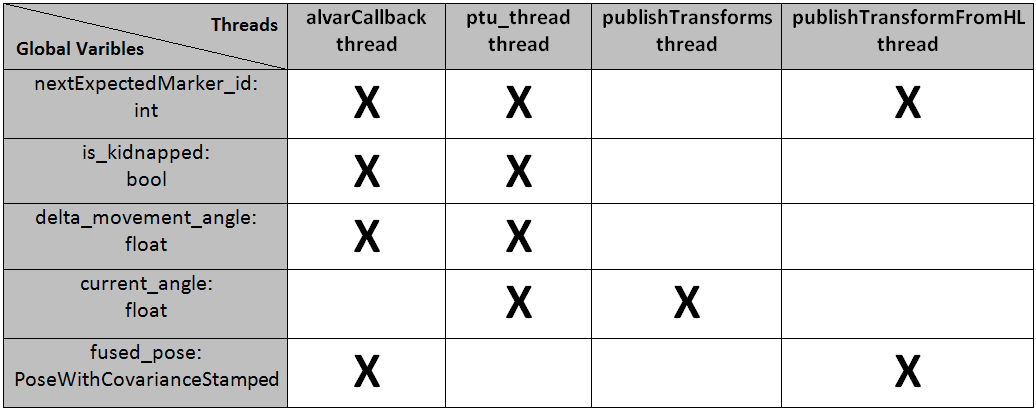
\includegraphics[width = \linewidth]{graphics/vision_threads.png}
\caption{Thread Communication}
\label{Thread Communication}
\end{center}
\end{figure}

\section{Problems and Challenges}

As already mentioned, there were as usually a lot problems practically from the start. But all of them are successfully resolved now and we have learned a lot from them. Here some of the problems we had will be briefly shown.

The first problem that confronted us was incorrect setup of the \texttt{ar\_track\_alvar} launch file, it was not meant to work with \texttt{freenect\_launch}, so we had to change the start connection between nodes, so that \texttt{ar\_track\_alvar} gets data from the Kinect. The next problem occurred when computing the covariance. The values we received from the algorithm were too inaccurate. We solved this problem by finding and implementing a queue with the right size of 25 samples, so the program has enough data in order to give back a usable covariance. After that we spent time thinking about the required size of the marker, so that we could maximize the distance from which Kinect will be able to see a marker. We tried bundles of markers, i.e. two and three markers on one, tried single markers and then settled with this solution since it is good enough for our needs.

Moreover we worked on the problem of positioning markers on the map (i.e. in the building), so that they are not too far away from each other and on the other hand so that there are not needlessly many of them on the map. Otherwise it would be irritating for the robot to see two markers at the same time. That problem was found while implementing an algorithm for the next expected marker.

Then, when working with PTU we had a problem developing the procedure to turn towards the expected marker. $atan$ is not defined at all locations, so at the end we used $atan2$, because it considers all special cases. Afterwards we had a problem with stopping the head when it was already looking in the marker's direction. We solved it by lowering accuracy for marker following. One of the last problems were the axes, that were not parallel to each other. We saw it in rviz and needed to dive into the code once again to find an error. The problem was found in the wrong implementation of the database. After we changed it, everything was working fine. 

\section{Testing}

Our first test was to find out how far the robot can go, while still being able to recognize the marker. We discovered that the viewing angle is approximately 58 degrees and viewing distance is 3.4 meters. Figure \ref{Field of View} visualizes the field of view.

After that we decided to put every marker on the wall within 2,5 meter distance. It turned out to yield good results. Then we worked on PTU movement to determine the optimal speed, so that it will neither turn too slow nor too fast. We came to the conclusion that 0,7 radians per second results in smooth and natural movement. Additionally we wrote a dummy program to verify that all values are interpreted as expected. By the time we ended up testing our software, we were practically done with our part of the project.

\begin{figure}
\begin{center}
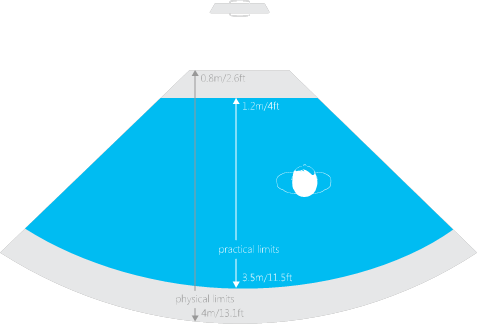
\includegraphics[scale=0.8]{graphics/view_field.png}
\caption{Field of View}
\label{Field of View}
\end{center}
\end{figure}
